\documentclass{beamer}

\usepackage[utf8]{inputenc}
\usepackage[T1]{fontenc}
\usepackage[spanish]{babel}
\usepackage{graphicx}
\usepackage{ragged2e}
\usepackage[table]{xcolor}
\usepackage{listings}
\usefonttheme[onlymath]{serif}

\definecolor{codegray}{rgb}{0.5,0.5,0.5}
\definecolor{backcolor}{rgb}{0.95,0.95,0.95}
\definecolor{verdecelda}{HTML}{B7CBA6}
\definecolor{rojocelda}{HTML}{FF9999}
\definecolor{lightgray}{gray}{0.6}


\usetheme{CambridgeUS}
\setbeamertemplate{navigation symbols}{}
\setbeamertemplate{blocks}[rounded][shadow=true]

\lstdefinestyle{mystyle}{
	backgroundcolor=\color{backcolor},
	commentstyle=\color{codegray},
	keywordstyle=\color{blue},
	numberstyle=\tiny\color{codegray},
	stringstyle=\color{red},
	basicstyle=\ttfamily\footnotesize,
	breaklines=true,
	captionpos=b,
	keepspaces=true,
	numbersep=5pt,
	showspaces=false,
	showstringspaces=false,
	showtabs=false,
	tabsize=2,
	inputencoding=utf8,
	extendedchars=true,
}

\lstset{style=mystyle}

\title{Trabajo Práctico 1}
\author{Cisnero, Seivane, Serafini}
\date{22 de Septiembre de 2025}

\begin{document}


\begin{frame}
	\centering
	
\includegraphics[width=0.25\textwidth]{UNAHUR (2)}
	\vfill
	{\huge \textbf{Trabajo Práctico 1}}\\[0.2cm]
	{\Large Aprendizaje Automático Avanzado}\\
	\vfill
	{\large Cisnero Matias, Seivane Nicolás, Serafini Franco}\\
	{\small 22 de Septiembre de 2025}
\end{frame}


\section{Ejercicio 1: Creación de Corpus}

\begin{frame}{}
	\centering
	\Large Ejercicio 1: Creación de Corpus\\
	\vspace{0.8cm}
	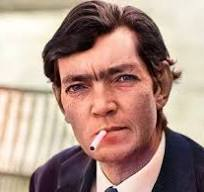
\includegraphics[width=0.5\textwidth]{imagen_cortazar}
\end{frame}
	
\begin{frame}[fragile]{1.1 Descripción de Librerías Usadas}
	
	\justifying
	Se utilizaron las librerías de $r$ y $pdfplumber$, en la cual utilizamos la ultima para leer página por página de un pdf y la primera para seleccionar las palabras.\\
	\vspace{0.1cm}
	Los links a las librerías son los siguientes.\\
	\vspace{0.1cm}
	\href{https://pypi.org/project/pdfplumber/#extracting-text}{\textbf{pdfplumber}}\\
	\vspace{0.1cm}
	\href{https://docs.python.org/es/3.13/library/re.html}{\textbf{r}}
	\vspace{0.2cm}
	
\begin{block}{Funciones Utilizadas}
	\begin{columns}[c]
		\column{0.45\textwidth}
		\begin{itemize}
			\item \texttt{pdfplumber.open() as pdf}
			\item \texttt{pdf.pages[]}
			\item \texttt{.extract\_text()}
			\item \texttt{.split('\textbackslash n')}
		\end{itemize}
		
		\column{0.45\textwidth}
		\begin{itemize}
			\item \texttt{re.findall()}
			\item \texttt{.endswith()}
			\item \texttt{.strip()}
			\item \texttt{.isdigit()}
			\item \texttt{.split('\textbackslash n')}
		\end{itemize}
	\end{columns}
\end{block}
	
\end{frame}

		%pdfplumber.open() = se utiliza para ir a la dirección del pdf, retornando una instancia de la% clase $pdfplumber.PDF$ 
%$pdf.pages[]$ = es una propiedad de la clase $pdfplumber.PDF$, la cual se puede indexar para acceder a %las paginas del pdf representadas en la clase $pdfplumber.Page$
%$.extract_text()$ = Método de la clase $pdfplumber.Page$, recopila todos los objetos de caracteres de %la página en un sol string.
%$split('\_n')$ = Divide el string que se genero antes en los saltos de pagina, generando una lista de %lineas.
%$re.findall()$ =
%$.endswith()$ =
%$.strip()$ =
%$.isdigit()$ =

\begin{frame}[fragile]{1.2.1 Estructura de Código}
	
	\justifying
	\textbf{\underline{Se utiliza la siguiente estructura de codigo:}}\\
	\vspace{0.1cm}
	Se comienza importando las librerías y creando una lista de palabras, donde se irán agregando las extracciones de texto.
	\begin{lstlisting}[language=Python]
import pdfplumber
import re

words = []
	\end{lstlisting}
	\justifying
	En lo cual se sigue utilizando la función \texttt{pdfplumber.open() as pdf}, en la cual se debe especificar la ruta hacia el pdf. El cual nos devuelve $pdf$ como una instancia de la clase \texttt{pdfplumber.PDF}
		\begin{lstlisting}[language=Python]
with pdfplumber.open("ruta") as pdf:
	\end{lstlisting}
\end{frame}

	
\begin{frame}[fragile]{1.2.2 Estructura de Código}
	
	\justifying
	Se continua utilizando una propiedad de la clase \texttt{pdfplumber.Page}, de la cual se puede indexar para acceder a las paginas del pdf
	\begin{lstlisting}[language=Python]
with pdfplumber.open("ruta") as pdf:
	for page in pdf.pages[:]:
	\end{lstlisting}
	\justifying
	En lo cual se utiliza el metodo \texttt{.extract\_text()}, que recopila todos los objetos de caracteres de la página en un solo string.
	\begin{lstlisting}[language=Python]
with pdfplumber.open("ruta") as pdf:
	for page in pdf.pages[:]:
		text = page.extract_text()
		if text:
	\end{lstlisting}
\end{frame}
	
\begin{frame}[fragile]{1.2.3 Estructura de Código}
	
	\justifying
	Se continua diviendo el string segun el metodo \texttt{.split('\textbackslash n')}, el cual devuleve una lista de strings, los cuales fueron separados de acuerdo a \textbackslash n, ergo saltos de linea.
	\begin{lstlisting}[language=Python]
with pdfplumber.open("ruta") as pdf:
	for page in pdf.pages[:]:
		text = page.extract_text()
			if text:
				lines = text.split('\n')
	\end{lstlisting}
	\justifying
	Luego se sacan las lineas que sean numeros de pagina tanto en el pie de la misma como en el encabezado. La forma de extraccion varia de acuerdo a como es el pdf.
	\begin{lstlisting}[language=Python]
				if lines[-1].strip().isdigit():
					lines = lines[:-1]
				if lines[0].strip().isdigit():
					lines = lines[1:]
				
	\end{lstlisting}
\end{frame}
	
\begin{frame}[fragile]{1.2.4 Estructura de Código}
	
	\justifying
	Se crea por linea una lista con el método de la librería r:\\
	\vspace{0.1cm}
	\texttt{re.findall(r"\_w+|[.,!?;:]", line)}, en el cual se separan con expresiones regulares las palabras con \textbackslash w+ y aparte los signos de puntuación con [.,!?;:], en una lista de strings. Luego para cada palabra se la pasa a minúscula con el método \texttt{.lower()}.
	\begin{lstlisting}[language=Python]
with pdfplumber.open("ruta") as pdf:
	for page in pdf.pages[:]:
		text = page.extract_text()
		if text:
			lines = text.split('\n')
			if lines[-1].strip().isdigit():
				lines = lines[:-1]
			if lines[0].strip().isdigit():
				lines = lines[1:]
			for line in lines:
				tokens = re.findall(r"\w+|[.,!?;:]", line)
				tokens = [token.lower() for token in tokens]
	\end{lstlisting}

\end{frame}

	
\begin{frame}[fragile]{1.2.5 Estructura de Código}
	
	\justifying
	Luego se diferencia por linea los puntos aparte, los cuales consideeramos los ultimos puntos de las lineas. Cada linea, las cuales fueron convertidas en listas de strings son agregadas a la lista del corpus\\

	\begin{lstlisting}[language=Python]
with pdfplumber.open("ruta") as pdf:
	for page in pdf.pages[:]:
		text = page.extract_text()
			if text:
				lines = text.split('\n')
				if lines[-1].strip().isdigit():
					lines = lines[:-1]
				if lines[0].strip().isdigit():
					lines = lines[1:]
				for line in lines:
					tokens = re.findall(r"\_w+|[.,!?;:]", line)
					tokens = [token.lower() for token in tokens]
				if line.endswith("."):
					tokens[-1]= ". "
				words.extend(tokens)
	\end{lstlisting}
	
	
%%% RAYUELA LOCOOOO	
	
	
	
\end{frame}
	
\begin{frame}{1.3 Libros utilizados: Rayuela}
	\justifying
	\textbf{Titulo:} Rayuela\\
	\textbf{Autor:} Julio Cortazar\\
	\textbf{Año :} 1963\\
	Se extrayeron 197.342 caracteres y 20.810 caracteres únicos que conforman el vocabulario.\\
	\centering
	\vspace{0.2cm}
	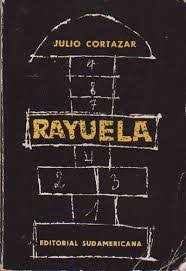
\includegraphics[width=0.3\textwidth]{rayuela_cortazar}
	
\end{frame}
	
\begin{frame}[fragile]{1.3.2 Código utilizado: Rayuela}
\begin{lstlisting}[language=Python]
with pdfplumber.open("Julio-Cortazar-Rayuela.pdf") as pdf:
	for page in pdf.pages[7:]:
		text = page.extract_text()
			if text:
				lines = text.split('\n')
				if lines[-1].strip().isdigit():
					lines = lines[:-1]
				if lines[0].strip().isdigit():
					lines = lines[1:]
				if lines[0].strip().isdigit():
					lines = lines[1:]
				if lines[-1].strip().isdigit():
					lines = lines[:-1]
				for line in lines:
					tokens = re.findall(r"\w+|[.,!?;:]", line)
					tokens = [token.lower() for token in tokens]
				if line.endswith("."):
					tokens[-1]= ". "
				words.extend(tokens)
\end{lstlisting}
	
\end{frame}
	
	
\begin{frame}{1.3.3 Ejemplo Borrado: Rayuela}
	\centering
	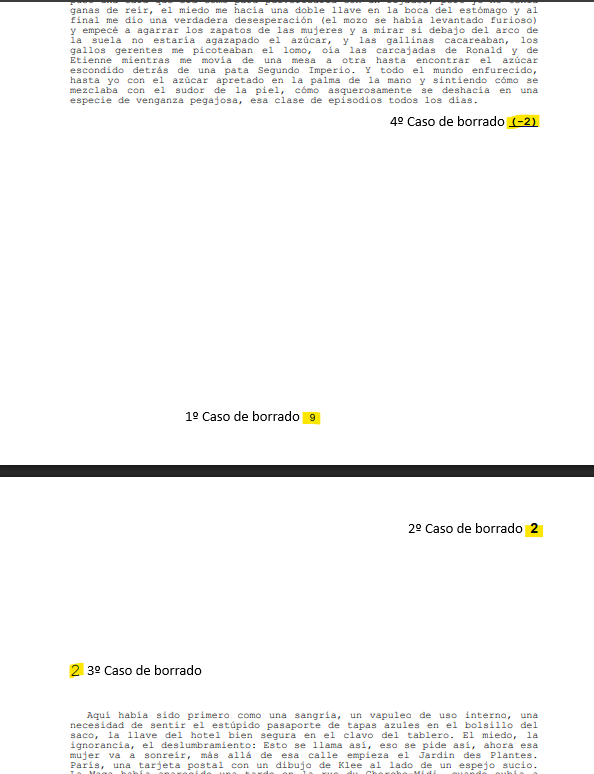
\includegraphics[width=0.5\textwidth]{borrado_rayuela}
	
\end{frame}	
	
	
%%% TODOS LOS FUEGOS

\begin{frame}{1.3 Libros utilizados: Todos los fuegos}
\justifying
\textbf{Titulo:} Todos los fuegos el fuego.\\
\textbf{Autor:} Julio Cortazar\\
\textbf{Año :} 1966\\
Se extrayeron 55.948 caracteres y 2.828 caracteres únicos que conforman el vocabulario.\\
\centering
\vspace{0.2cm}
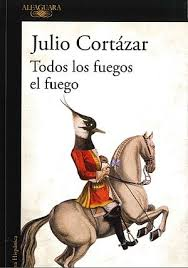
\includegraphics[width=0.3\textwidth]{todos_los_fuegos_cortazar}

\end{frame}

\begin{frame}[fragile]{1.3.2 Código utilizado: Todos los fuegos}
\begin{lstlisting}[language=Python]
with pdfplumber.open("Julio Cortazar Todos los fuegos.pdf") as pdf:
	for page in pdf.pages[:-1]:
		text = page.extract_text()
			if text:
				lines = text.split('\n')
				if lines[-1].strip().isdigit():
					lines = lines[:-1]
				for line in lines:
					tokens = re.findall(r"\w+|[.,!?;:]", line)
					tokens = [token.lower() for token in tokens]
				if line.endswith("."):
					tokens[-1]= ". "
				words.extend(tokens)
		\end{lstlisting}

\end{frame}


\begin{frame}{1.3.3 Ejemplo Borrado: Todos los fuegos}
\centering
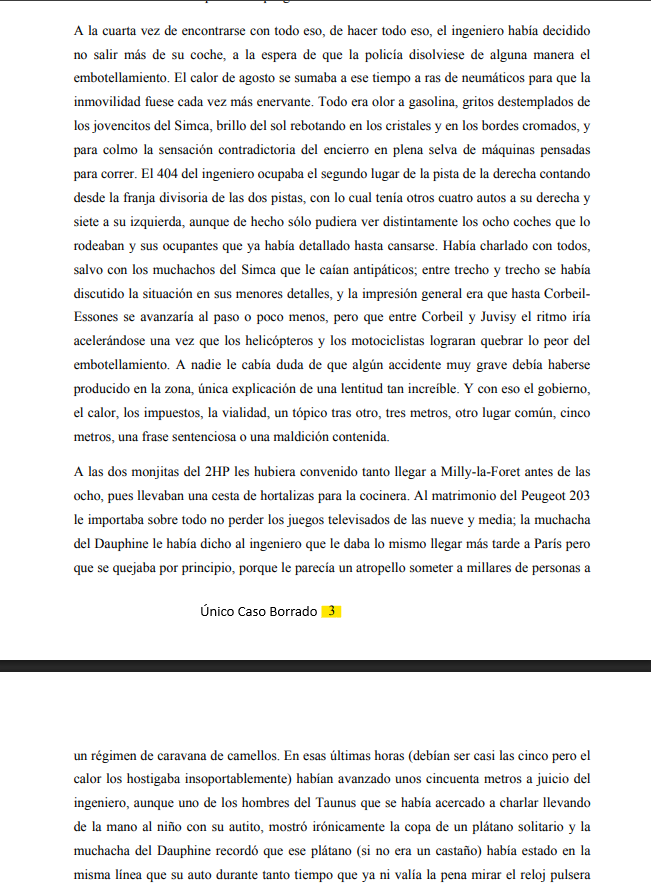
\includegraphics[width=0.5\textwidth]{borrado_todoslosfuegos}

\end{frame}	
	
%%% un tal lucas

\begin{frame}{1.3 Libros utilizados: Historias de cronopios y de famas}
	\justifying
	\textbf{Titulo:} Historias de cronopios y de famaso.\\
	\textbf{Autor:} Julio Cortazar\\
	\textbf{Año :} 1962\\
	Se extrayeron 32.224 caracteres y 2.514 caracteres únicos que conforman el vocabulario.\\
	\centering
	\vspace{0.2cm}
	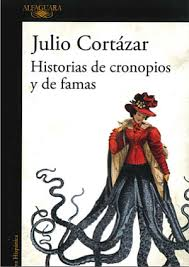
\includegraphics[width=0.3\textwidth]{historias_de_cronopios_y_de_famas_cortazar}
	
\end{frame}

\begin{frame}[fragile]{1.3.2 Código utilizado: Historias de cronopios y de famas}
	\justifying
	En este caso no fue necesario quitar ninguna linea.
	\begin{lstlisting}[language=Python]
with pdfplumber.open("Historias-de-Cronopios-y-de-Famas - Julio Cortazar.pdf") as pdf:
	for page in pdf.pages[3:-1]:
		text = page.extract_text()
			if text:
				lines = text.split('\n')
				for line in lines:
					tokens = re.findall(r"\w+|[.,!?;:]", line)
					tokens = [token.lower() for token in tokens]
				if line.endswith("."):
					tokens[-1]= ". "
				words.extend(tokens)
	\end{lstlisting}
	
\end{frame}
	
	
%% ahora si un tal lucas

\begin{frame}{1.3 Libros utilizados: Un tal Lucas.}
	\justifying
	\textbf{Titulo:} Un tal Lucas.\\
	\textbf{Autor:} Julio Cortazar\\
	\textbf{Año :} 1979\\
	Se extrayeron 32.224 caracteres y 2.514 caracteres únicos que conforman el vocabulario.\\
	\centering
	\vspace{0.2cm}
	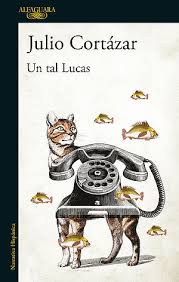
\includegraphics[width=0.3\textwidth]{un_tal_lucas_cortazar}
	
\end{frame}

\begin{frame}[fragile]{1.3.2 Código utilizado: Un tal Lucas.}
	\begin{lstlisting}[language=Python]

with pdfplumber.open("Lucas_Julio_Cortazar.pdf") as pdf:
	for page in pdf.pages[5:]:
		text = page.extract_text()
			if text:
				lines = text.split('\n')
				if lines[-1].strip().isdigit():
					lines = lines[:-1]
				lines = lines[1:]
				for line in lines:
					tokens = re.findall(r"\w+|[.,!?;:]", line)
					tokens = [token.lower() for token in tokens]
				if line.endswith("."):
					tokens[-1]= ". "
				words.extend(tokens)
	\end{lstlisting}
	
\end{frame}


\begin{frame}{1.3.3 Ejemplo Borrado: Un tal Lucas.}
	\centering
	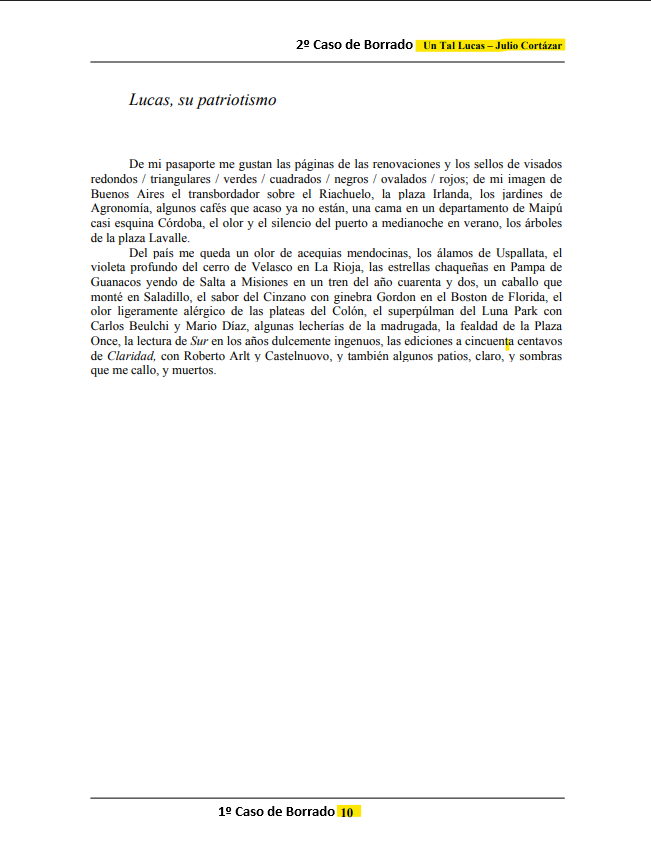
\includegraphics[width=0.5\textwidth]{borrado_un_tal_lucas}
\end{frame}	
	
	
\begin{frame}[fragile]{1.4 Corpus final}
	\justifying
	Se guarda el corpus final en un archivo llamado \textbf{corpus.txt}.
	
	\begin{lstlisting}[language=Python]
		with open("corpus.txt", "w", encoding="utf-8") as f:
			f.write("\n".join(words))
	\end{lstlisting}
	
	Obteniendo un corpus como se ve en la siguiente imagen.
	\vspace{0.1cm}
\begin{columns}[t] % [t] para alinear arriba
	\column{0.55\textwidth}
	\textbf{Vocabulario (único):} 27.971\\
	\textbf{Corpus total:} 310.347
	
	\column{0.45\textwidth}
	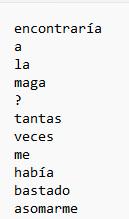
\includegraphics[width=0.5\linewidth]{corpus_txt.png}
\end{columns}

\end{frame}


\section{Ejercicio 2: Implementación CBOW y SkipGram}

\begin{frame}{}
	\centering
	\Large Ejercicio 2: Implementación CBOW y SkipGram\\
	\vspace{0.8cm}
	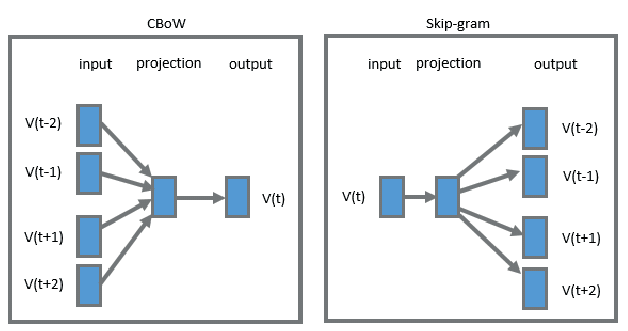
\includegraphics[width=0.5\textwidth]{imagenes_cbow_skipgram}
\end{frame}



	
\begin{frame}[fragile]{2.1 Pasos previos}
	\justifying
	Se abre y carga el \textbf{corpus.txt}.
	
	\begin{lstlisting}[language=Python]
with open("corpus.txt", "r", encoding="utf-8") as f:
	corpus = f.read().splitlines()
	\end{lstlisting}
	Luego se crean los diccionarios que se utilizaran en ambos métodos.
	\begin{lstlisting}[language=Python]
    vocab = sorted(set(corpus))
		vocab_tamano = len(vocab)
		palabra_a_indice = {palabra: i for i, palabra in enumerate(vocab)}
		indice_a_palabra = {i: palabra for i, palabra in enumerate(vocab)}
	\end{lstlisting}

\end{frame}
	
\begin{frame}[fragile]{2.2 CBOW}
	\begin{block}{\textbf{Definición:} Continuous Bag of Words(CBOW)}
	\justifying
	\vspace{0.1cm}
	\textbf{Propósito:} Es un modelo de aprendizaje automático para aprender representaciones de palabras que capturan el "significado" de las palabras basadas en su contexto.\\
	\vspace{0.1cm}
	\textbf{Principio:} A diferencia de los modelos más simples, CBOW utiliza un contexto de $C$ palabras para predecir una palabra central\\
	\vspace{0.1cm}
	\textbf{Contexto vs. Predicción:}  A partir de un contexto de $C$ palabras ($p_{I,1}, p_{I,2}, ..., p_{I,C}$), se intenta predecir la palabra objetivo ($p_O$), que generalmente es la palabra central
	\end{block}
	
\end{frame}
	
	
	
\begin{frame}[fragile]{X.X Skip-gram}
	\begin{block}{\textbf{Definición:} Skip-gram}
		\justifying
		\vspace{0.1cm}
		\textbf{Propósito:} Es un modelo de aprendizaje automático para aprender representaciones de palabras que capturan el significado de las palabras basadas en su contexto. La diferencia con CBOW es que la entrada de la red es una palabra y la salida intenta predecir su contexto.\\
		\vspace{0.1cm}
		\textbf{Principio:} Skip-gram utiliza una palabra central para predecir un contexto de C palabras.\\
		\vspace{0.1cm}
		\textbf{Contexto vs. Predicción:} A partir de una palabra central ($p_O$), el modelo intenta predecir las palabras de su contexto ($p_{I,1}, p_{I,2}, ..., p_{I,C}$).
	\end{block}    
\end{frame}

\begin{frame}[fragile]{X.X Skip-gram}
	\centering
	\Large Arquitectura de Skip-gram
	\vspace{0.5cm} 
	\vfill
	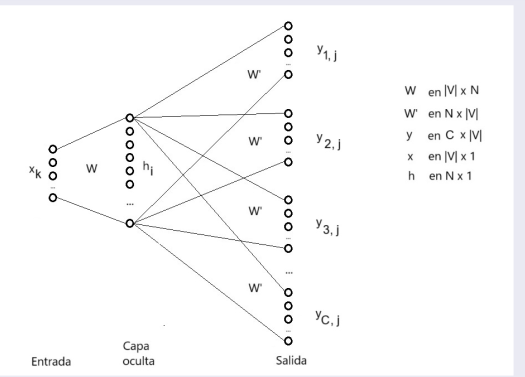
\includegraphics[width=0.6\textwidth]{Skip_arq.png}
	\vfill
\end{frame}

\begin{frame}[fragile]{X.X Skip-gram: Representación de la entrada}
	\begin{block}{\textbf{Entrada del modelo}}
		\justifying
		\textbf{Palabra central:} se representa como un vector one-hot $x \in \mathbb{R}^{|V|}$, 
		donde $|V|$ es el tamaño del vocabulario.\\
		\vspace{0.2cm}
		Ejemplo: si $|V|=10\,000$ y la palabra central ocupa la posición 125, 
		entonces $x$ tiene un 1 en la posición 125 y 0 en las demás.\\
		\vspace{0.2cm}
		\textbf{Matriz de embeddings de entrada:} 
		\[
		W \in \mathbb{R}^{|V| \times N}
		\]
		donde $N$ es la dimensión del espacio de embeddings (ej. $N=300$).
	\end{block}
\end{frame}

\begin{frame}[fragile]{X.X Skip-gram: Representación vectorial}
	\begin{block}{\textbf{Cálculo de la representación vectorial de la palabra $p_I$}}
		\justifying
		La capa oculta no tiene función de activación. 
		Se obtiene directamente el embedding de la palabra central:
		\[
		h = W^T x = v_{p_I}, \quad h \in \mathbb{R}^N
		\]
		donde $v_{p_I}$ es el vector de embeddings asociado a la palabra central $p_I$.\\
		\vspace{0.2cm}
		Dimensiones:
		\begin{itemize}
			\item $x \in \mathbb{R}^{|V|}$ (one-hot).
			\item $W \in \mathbb{R}^{|V| \times N}$.
			\item $h \in \mathbb{R}^N$ (embedding resultante).
		\end{itemize}
	\end{block}
\end{frame}

\begin{frame}[fragile]{X.X Skip-gram: Salida y softmax}
	\begin{block}{\textbf{Cálculo de probabilidades}}
		\justifying
		Para cada palabra candidata $j$ en el vocabulario, se calcula:
		\[
		u_j = (v'_j)^T h, \qquad u \in \mathbb{R}^{|V|}
		\]
		donde $v'_j$ es el vector de salida correspondiente a la palabra $j$, 
		y $W' \in \mathbb{R}^{N \times |V|}$ es la matriz de salida.\\
		\vspace{0.2cm}
		Luego se aplica softmax:
		\[
		y_j = \frac{\exp(u_j)}{\sum_{k=1}^{|V|} \exp(u_k)}
		\]
		obteniendo la probabilidad de que la palabra $j$ aparezca en el contexto de $p_I$.
	\end{block}
\end{frame}

\begin{frame}[fragile]{X.X Skip-gram: Función de pérdida}
	\begin{block}{\textbf{Pérdida logarítmica}}
		\justifying
		Dado un contexto de $C$ palabras alrededor de la palabra central $p_I$, 
		la función de pérdida se define como:
		\[
		E = - \sum_{c=1}^{C} \log P(p_{O_c} \mid p_I)
		\]
		donde $p_{O_c}$ son las palabras del contexto.\\
		\vspace{0.2cm}
	\end{block}
\end{frame}

\begin{frame}[fragile]{X.X Skip-gram: Actualización}
	\begin{block}{\textbf{Reglas de actualización}}
		\justifying
		Durante el entrenamiento, los vectores de entrada y salida se ajustan.\\
		\vspace{0.2cm}
		Para los vectores de salida:
		\[
		v'_j \leftarrow v'_j - \eta \, E_{Ij} \, h
		\]
		Para el vector de entrada de la palabra central:
		\[
		v_{p_I} \leftarrow v_{p_I} - \eta \, EH^T
		\]
		donde:
		\begin{itemize}
			\item $\eta$ es la tasa de aprendizaje.
			\item $E_{Ij}$ depende del error para cada palabra del contexto.
		\end{itemize}
	\end{block}
	
\end{frame}


	
	
	
\end{document}